\documentclass[14Q,twocolumn]{jsarticle}
\usepackage[dvipdfmx]{graphicx}
\usepackage{wrapfig}
\usepackage{float}
\usepackage{otf}
\usepackage{longtable}
\usepackage{ulem}
\usepackage{ascmac}
\usepackage{multicol}
%%%%%
\makeatletter
\newenvironment{tablehere}
  {\def\@captype{table}}
  {}
\newenvironment{figurehere}
  {\def\@captype{figure}}
  {}
\makeatother
%%%%%%
\setlength{\textwidth}{160truemm}      % テキスト幅: 160mm
\setlength{\fullwidth}{\textwidth}     % ページ全体の幅
\setlength{\oddsidemargin}{0mm}   % 左余白
\setlength{\topmargin}{-10mm}       % 上余白
\setlength{\textheight}{240truemm}     % テキスト高さ: 297-(30+30)=237mm
\pagestyle{empty}
\title{紙地図をGISで使う}% 文書のタイトル
\date{2018年9月18日}
\author{厚沢部町 石 井 淳 平}              % 著者

%------------------------------
\begin{document}
\maketitle
%\begin{multicols}{2}
\section{この時間に覚えること}
\begin{itemize}
\item ジオリファレンサーを使って紙図面に座標を与える。
\item 変換方法やリサンプリングについて知る。
\end{itemize}


%%%%
\section{作業の流れ}
\begin{enumerate}
\item ラスタ→ジオリファレンサー→ジオリファレンサー
\item ファイル→ラスタを開く
\item ジオリファレンサーに紙図面を読み込み
\item グリッド交点をクリックしてポイント追加
\item 交点座標を入力するか、背景図から座標を取得
\item 同一地点をクリックして座標を取得
\end{enumerate}

\section{座標を取得する}
図面に座標を与えるために、紙地図の特定の地点の座標を取得します。座標の取得方法は2通りあり、紙地図の特定の地点の座標がわかっている場合(発掘調査図面でグリッド交点の座標がわかっている場合など)はX座標、Y座標を手入力します。紙地図上で座標が明らかではない場合(国土地理院の旧版地形図や航空写真の場合)には、紙地図とすでにGISデータになっている別の図面の同一地点を比定して座標を取得します。

背景地図にはGoogleMapや地理院地図などのウェブ地図も使用できます。

\begin{figurehere}
\centering
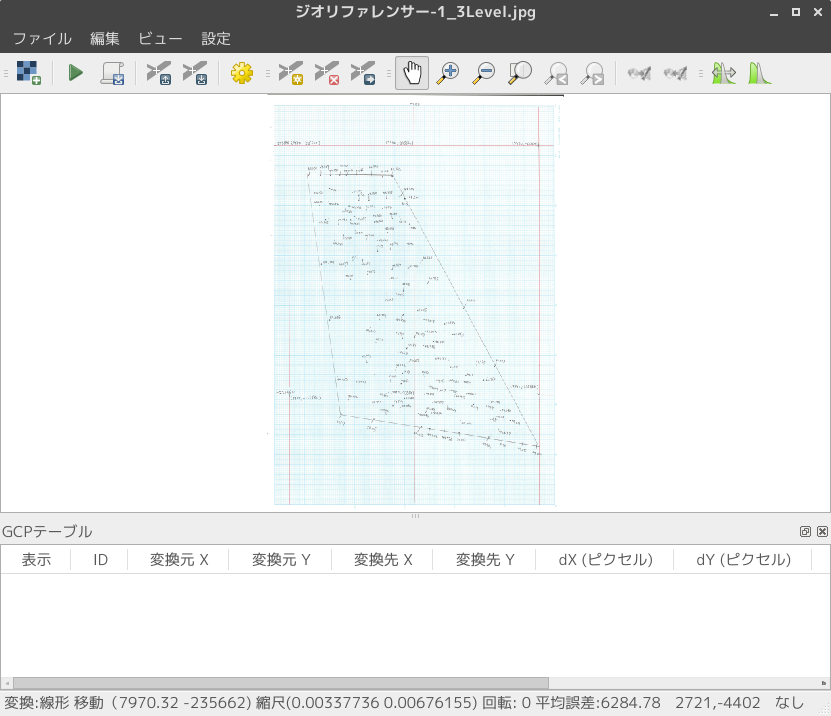
\includegraphics[width=0.8\linewidth]{04.png}
\caption{ジオリファレンサーの起動}
\end{figurehere}

\begin{figurehere}
\centering
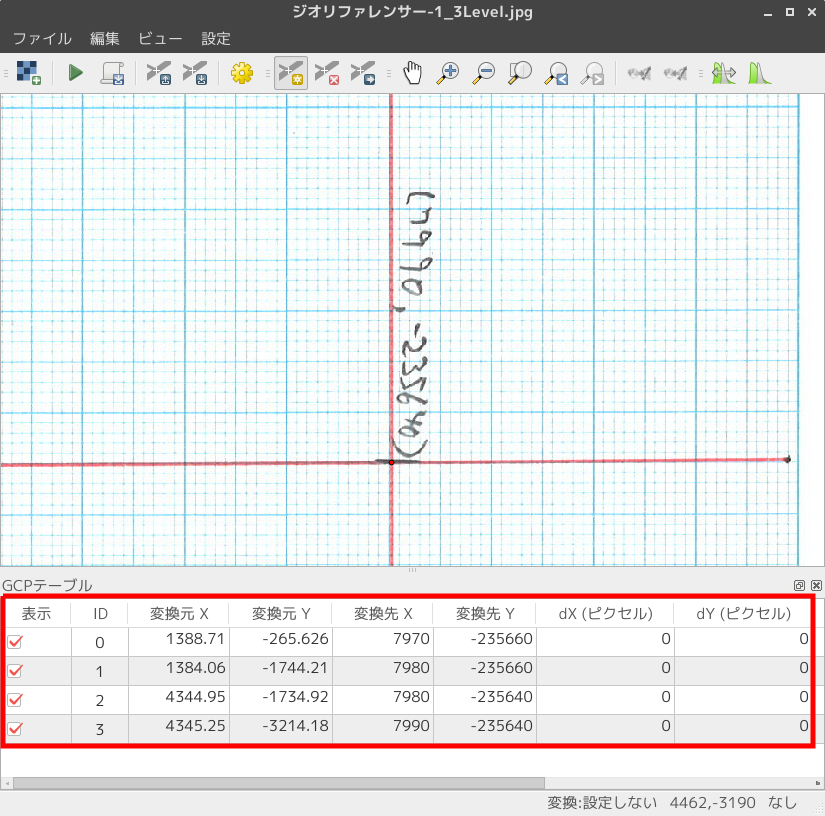
\includegraphics[width=0.8\linewidth]{10.png}
\caption{ジオリファレンサーで座標を取得}
\end{figurehere}


\section{幾何補正のコツ}
幾何補正を正確に行うためには、同一地点の正確な比定と適切なGCPポイント\footnote{
GCPポイントは座標を付与する点のことです。
}の設置が必要です。正確に設置されたGCPポイントの周辺では幾何補正の精度が高くなりますが、GCPポイントから離れると補正量が増加し精度が下がっていきます。このため、GCPポイントの数とばらつき具合が重要となります。GCPポイントはある程度までは多いほうが精度が上がりますが、一定数以上\footnote{
GCPポイントの適切な数がどのくらいか、ということはなかなか確定できませんが、A4サイズでスキャンした紙図面の場合、15点くらいまでは精度が上がっていくようですが、それ以上になると苦労の割に精度が上がらないようです。また、GCPポイントが増えると比定地のズレが累積することも、単純にGCPポイントが増えれば精度が上がる結果に繋がらないようです。
}
増やしても精度にはつながらないようです。

GCPポイントの目安として次のことを心がけています。

\begin{itemize}
\item 1図面につき6点をめざす。
\item なるべく図面全体をまんべんなくカバーするように設置する。
\item 6点設置したところで一度幾何補正を実行し、追加のGCPポイントの必要性を判断する。
\end{itemize}

\section{変換タイプ}
たくさんの変換タイプが用意されていますが、「線形」か「シンプレートスプライン」で試してみてください。
\begin{itemize}
\item 線形
\item ヘルマート
\item 多項式1
\item 多項式1
\item 多項式1
\item シンプレートスプライン
\item 投影変換
\end{itemize}

\section{リサンプリング方法}
迷ったら、「線形」で試してみてください。

\begin{itemize}
\item 最近傍
\item 線形
\item キュービック
\item キュービックスプライン
\item ランチョシュ
\end{itemize}

リサンプリング方法については対象となるラスタデータの性質\footnote{
地形分類図や植生図などをラスタ化して統計的な演算処理をする場合などではリサンプリングによってデータ値が変化しては困ります。例えば植生図でブナ林を赤にナラ林を青に割り当てた場合、ナラ林とブナ林の中間に赤と青の中間色が補完されてしまうと意味がなくなってしまいます。「最近傍」によるリサンプリングではこうしたデータの間を埋める処理を行わないようにします。一方、航空写真のような「絵」として意味があるデータでは隣接するピクセルが滑らかに連続していることが必要です。「キュービック」によるリサンプリングではデータの中間値を適切に処理して滑らかな絵を作成します。
}
によって使い分ける場合もあります。

離散的なデータでは統計的な変化がない「最近傍」、なめらかにデータを保管したい航空写真では「キュービック」を選択しておけばよいでしょう。

\section{変換先SRS}
よく利用するEPSGコードを覚えておくと作業がはかどります。おもな測地系、座標系は次のようなものです。
\begin{itemize}
\item 日本測地系(Tokyo Datam)
	\begin{itemize}
	\item 緯度経度系(4301)
	\item 平面直角座標系(30161〜30179)
	\item ユニバーサルトランスバースメルカトルグリッド(102151〜102156)
	\end{itemize}
\item 世界測地系(JGD2000)
	\begin{itemize}
	\item 緯度経度系(4612)
	\item 平面直角座標系(2443〜2461)
	\item ユニバーサルトランスバースメルカトルグリッド (3097〜3101)
	\end{itemize}
\item WGS84(4326)
\end{itemize}

\begin{figurehere}
\centering
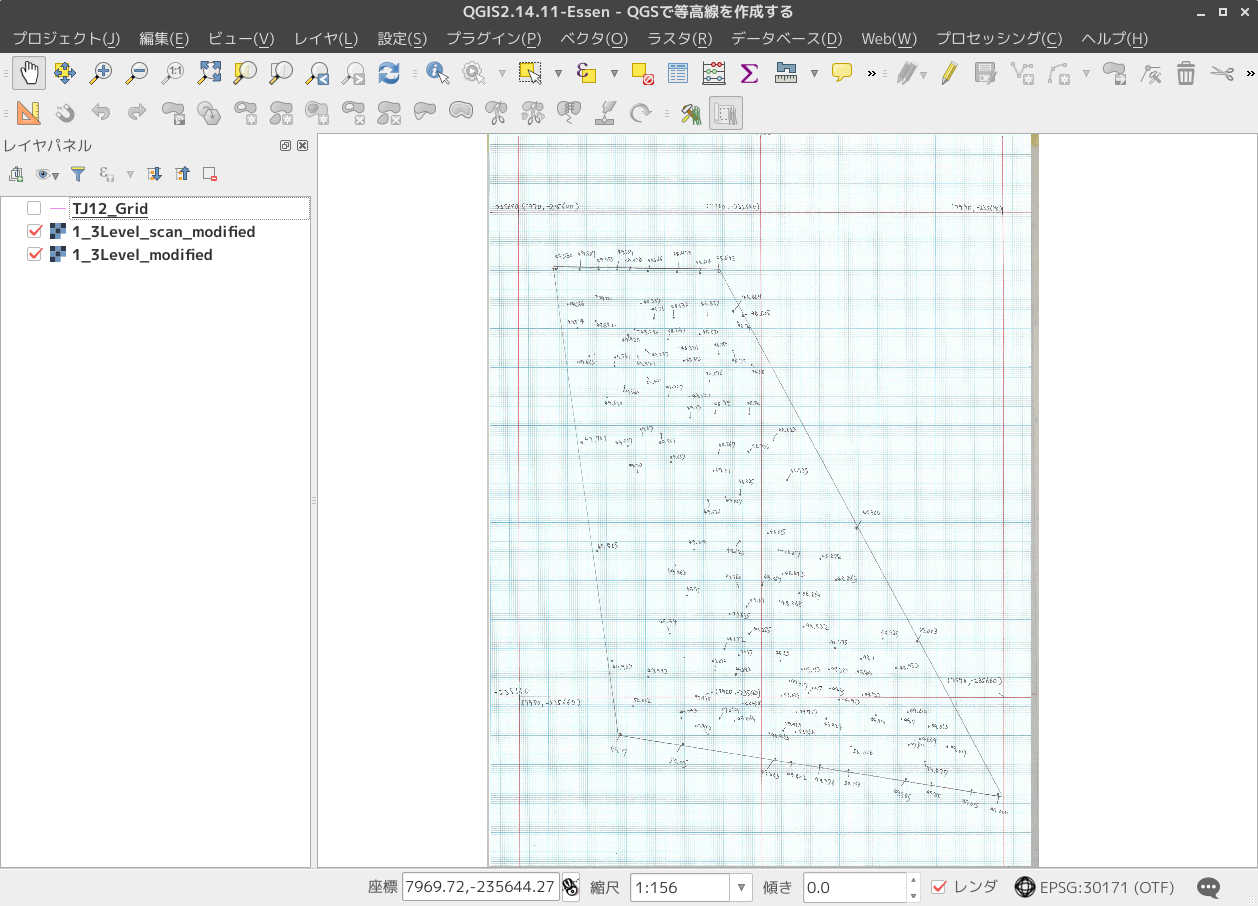
\includegraphics[width=0.8\linewidth]{16.png}
\caption{幾何補正されてGISデータ化された紙地図}
\end{figurehere}

%%%%
\section{幾何補正された図面}
幾何補正された紙地図はラスタデータとして扱うことができます。航空写真や旧版地図などのように画像として利用する場合もありますが、トレースしてベクタデータを生成する際の原図として利用することもあります。

\begin{figurehere}
\centering
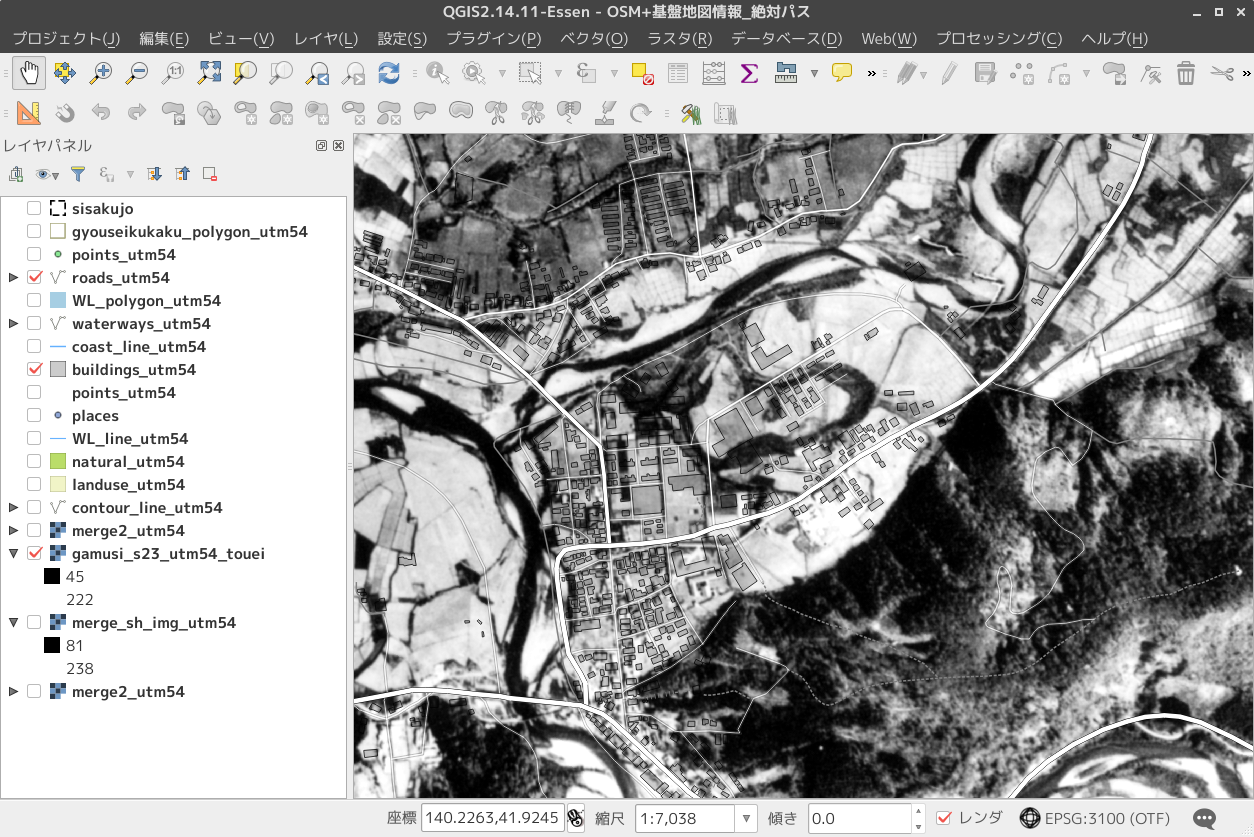
\includegraphics[width=1\linewidth]{17.png}
\caption{幾何補正された米軍撮影航空写真(\copyright 国土地理院)}
\end{figurehere}

\begin{figurehere}
\centering
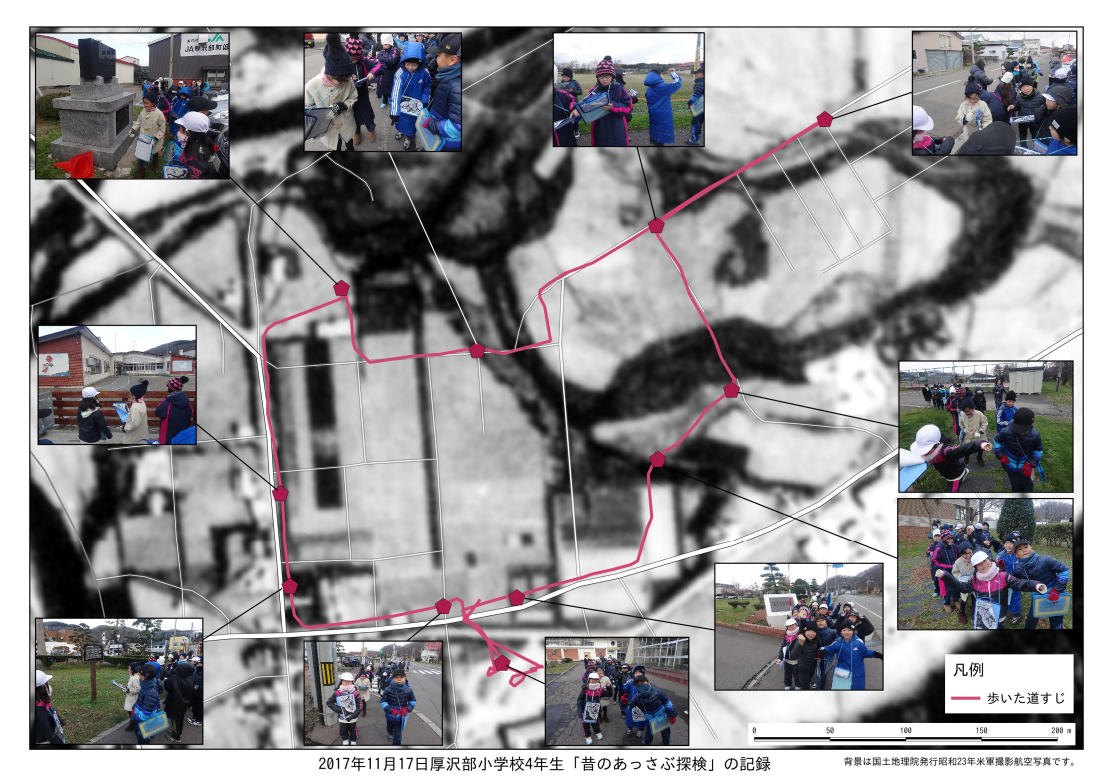
\includegraphics[width=1\linewidth]{17-2.png}
\caption{幾何補正された航空写真を利用したフィールドワーク}
\end{figurehere}

\begin{figurehere}
\centering
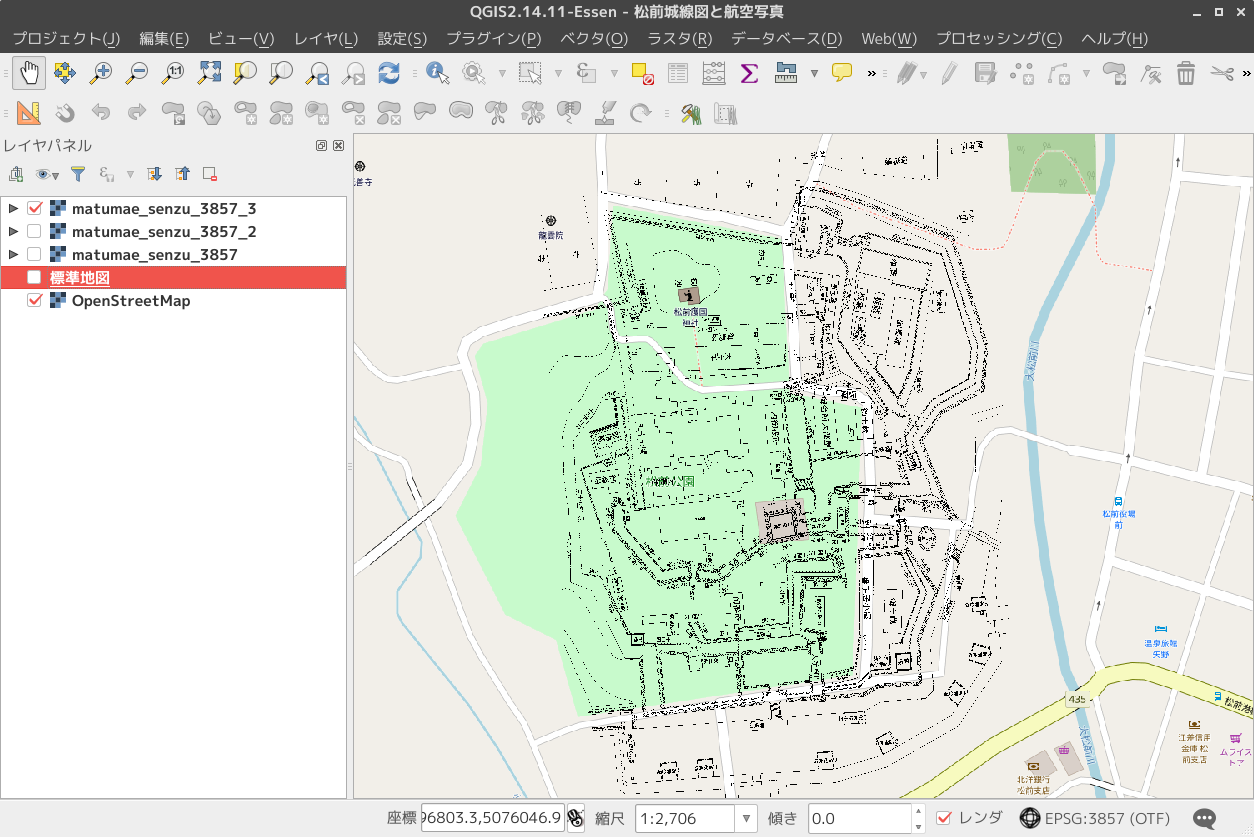
\includegraphics[width=1\linewidth]{18.png}
\caption{ウェブ地図と縄張り図}
\end{figurehere}

%%%
\section{図面を取り込む手法}
幾何補正を行うためには図面をデジタル化する必要があります。発掘調査で作成される現場図面のサイズはB3が標準です。このサイズの図面を一度にスキャンできる環境はあまり多くないと思われます。大判の紙図面をデジタル化する方法は次の2点が考えられます。

\begin{enumerate}
\item A3あるいはA4に縮小コピーした現場図面をスキャンする。
\item 現場図面を写真撮影する。
\end{enumerate}

実際に試したところ、縮小コピーしてスキャンする方が精度は高くなりますが、長焦点のレンズを使用した場合には写真撮影でも十分実用に耐える精度が確保できるようです。時間と機材にあわせて選択してください。

\begin{figurehere}
\centering
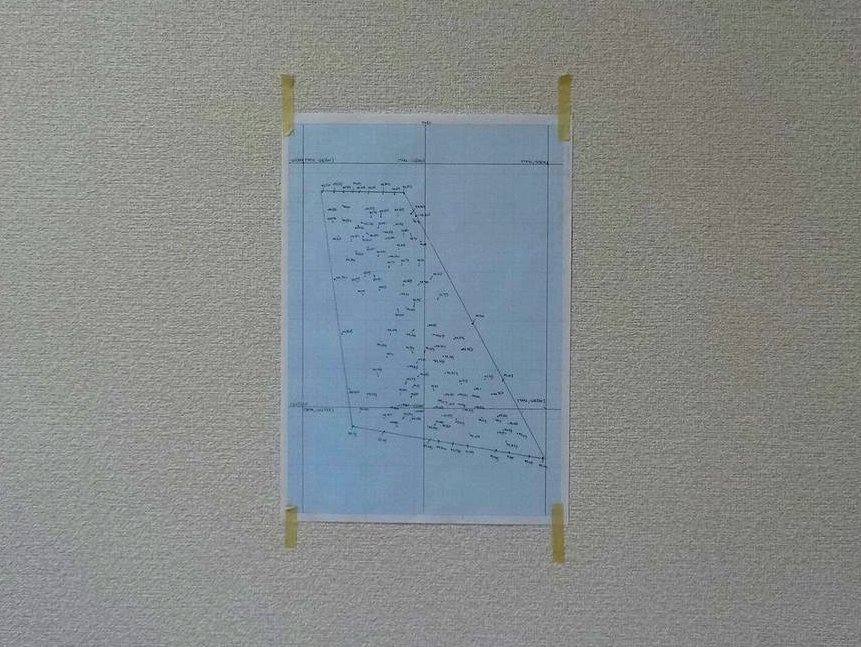
\includegraphics[width=1\linewidth]{19.jpg}
\caption{現場図面を撮影してデジタル化}
\end{figurehere}

%\end{multicols}
\end{document}
